\section{Experimentos de qualidade}
\label{sec:experimentos-qualidade}
A heurística desenvolvida foi aplicada a alguns gráficos clássicos da
literatura, com o objetivo de avaliar o quão próximo da CMV a
cobertura de vértices produzida fica.

Para cada exemplo, serão apresentados o grafo, junto com a
CMV do mesmo. Além disso, serão apresentados três números:
\begin{description}
    \item[$n$] O número de vértices do grafo.
    \item[$k$] O número de vértices da CMV.
    \item[$k'$] O número de vértices da cobertura de vértices
    encontrada pela heurística.
\end{description}

\subsection{O tetraedro}
Para o tetraedro~\cite{cite:example-plato},
apresentado na Figura~\ref{fig:example-tetraedro}.

\begin{figure}[htb]
\centering
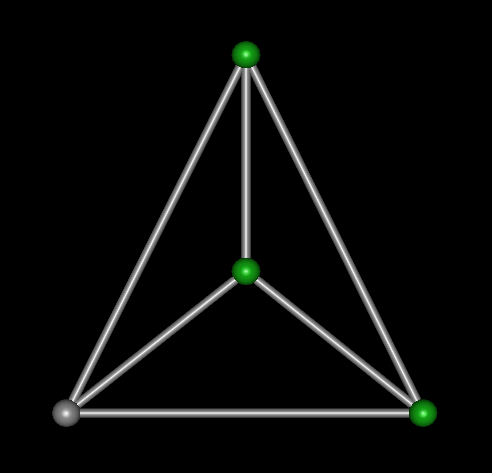
\includegraphics[width=0.4\textwidth]{img/tetraedro.png}
\caption{Tetraedro, $n=4$, $k=3$, $k'=3$}
\label{fig:example-tetraedro}
\end{figure}

\subsection{O grafo bipartido de Kuratowski $K_{3,3}$}
Para o grafo bipartido de Kuratowski
$K_{3,3}$~\cite{cite:example-kuratowski},
apresentado na Figura~\ref{fig:example-kuratowski}.

\begin{figure}[htb]
\centering
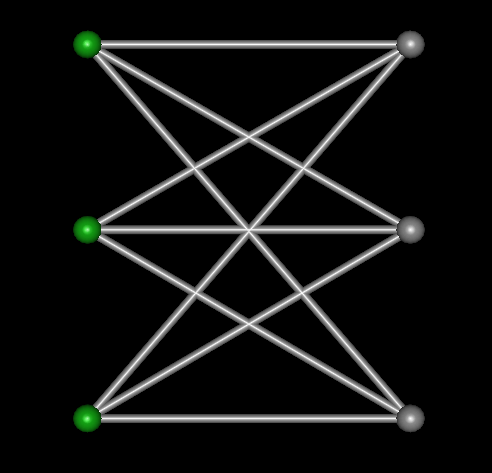
\includegraphics[width=0.4\textwidth]{img/kuratowski.png}
\caption{Grafo bipartido de Kuratowski $K_{3,3}$, $n=6$, $k=3$, $k'=3$}
\label{fig:example-kuratowski}
\end{figure}


\subsection{O octaedro}
Para o octaedro~\cite{cite:example-plato},
apresentado na Figura~\ref{fig:example-octaedro}.

\begin{figure}[htb]
\centering
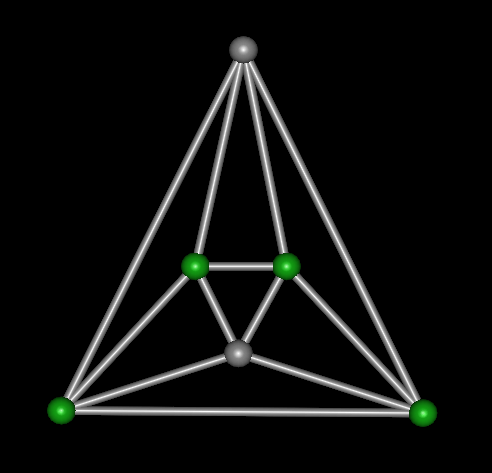
\includegraphics[width=0.4\textwidth]{img/octaedro.png}
\caption{Octaedro, $n=6$, $k=4$, $k'=4$}
\label{fig:example-octaedro}
\end{figure}


\subsection{O grafo de Bondy-Murphy $G_1$}
Para o grafo de Bondy-Murphy $G_1$~\cite{cite:example-bondy},
apresentado na Figura~\ref{fig:example-bondymurphyg1}.

\begin{figure}[htb]
\centering
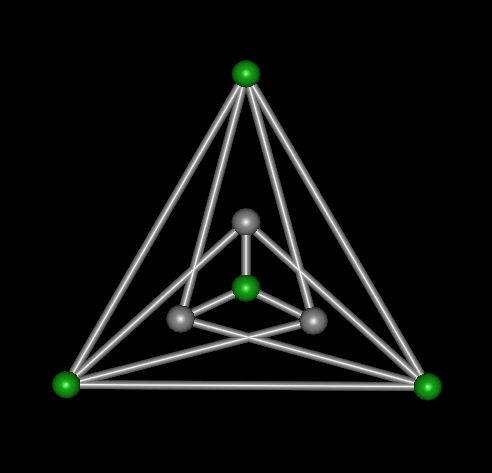
\includegraphics[width=0.4\textwidth]{img/bondymurphyg1.png}
\caption{Grafo de Bondy-Murphy $G_1$, $n=7$, $k=4$, $k'=4$}
\label{fig:example-bondymurphyg1}
\end{figure}


\subsection{O grafo roda $W_8$}
Para o grafo roda $W_8$~\cite{cite:example-bondy},
apresentado na Figura~\ref{fig:example-wheel}.

\begin{figure}[htb]
\centering
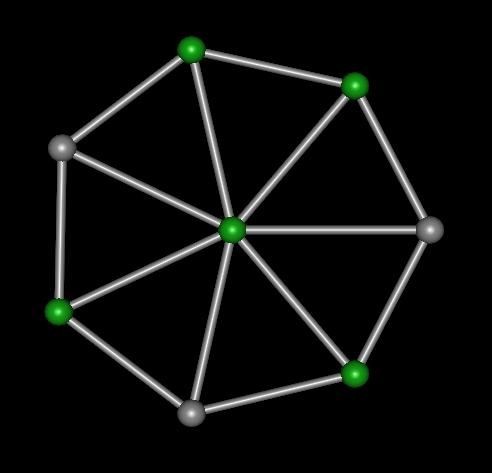
\includegraphics[width=0.4\textwidth]{img/wheel.png}
\caption{Grafo roda $W_8$, $n=8$, $k=5$, $k'=5$}
\label{fig:example-wheel}
\end{figure}


\subsection{O cubo}
Para o grafo cubo~\cite{cite:example-plato},
apresentado na Figura~\ref{fig:example-cube}.

\begin{figure}[htb]
\centering
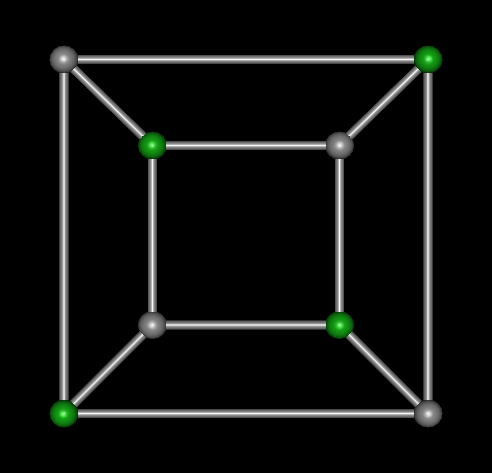
\includegraphics[width=0.4\textwidth]{img/cube.png}
\caption{Grafo cubo, $n=8$, $k=4$, $k'=4$}
\label{fig:example-cube}
\end{figure}


\subsection{O grafo Petersen}
Para o grafo Petersen~\cite{cite:example-petersen},
apresentado na Figura~\ref{fig:example-petersen}.

\begin{figure}[htb]
\centering
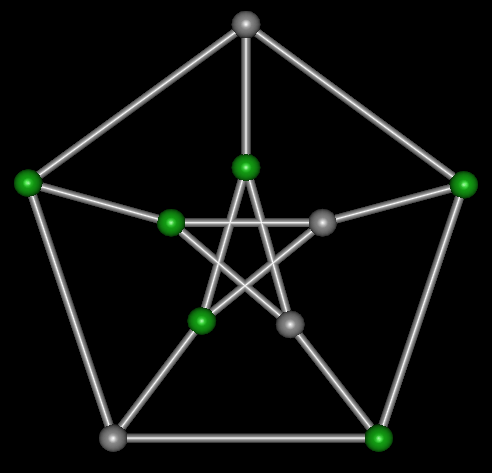
\includegraphics[width=0.4\textwidth]{img/petersen.png}
\caption{Grafo de Petersen, $n=10$, $k=6$, $k'=6$}
\label{fig:example-petersen}
\end{figure}


\subsection{O grafo de Bondy-Murphy $G_2$}
Para o grafo de Bondy-Murphy $G_2$~\cite{cite:example-bondy},
apresentado na Figura~\ref{fig:example-bondymurphyg2}.

\begin{figure}[htb]
\centering
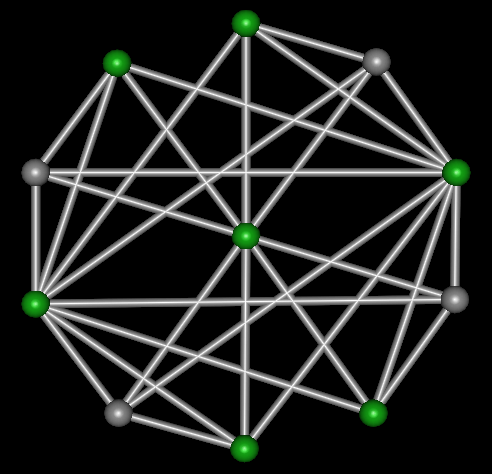
\includegraphics[width=0.4\textwidth]{img/bondymurphyg2.png}
\caption{Grafo de Bondy-Murphy $G_2$, $n=11$, $k=7$,$k'=7$}
\label{fig:example-bondymurphyg2}
\end{figure}


\subsection{O grafo de Grötzsch}
Para o grafo de Grötzsch~\cite{cite:example-grotzsch},
apresentado na Figura~\ref{fig:example-grotzsch}.

\begin{figure}[htb]
\centering
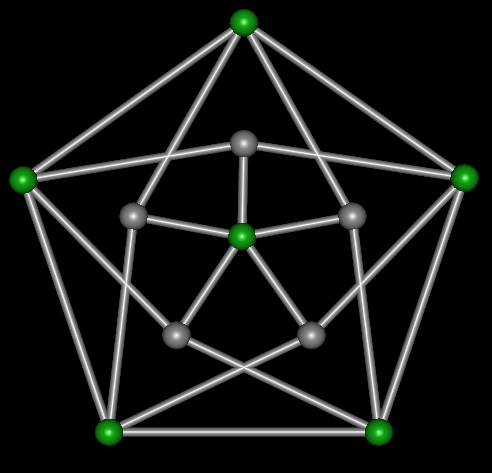
\includegraphics[width=0.4\textwidth]{img/grotzsch.png}
\caption{Grafo de Grötzsch, $n=11$, $k=6$, $k'=6$}
\label{fig:example-grotzsch}
\end{figure}


\subsection{O grafo de Herschel}
Para o grafo de Herschel~\cite{cite:example-herschel},
apresentado na Figura~\ref{fig:example-herschel}.

\begin{figure}[htb]
\centering
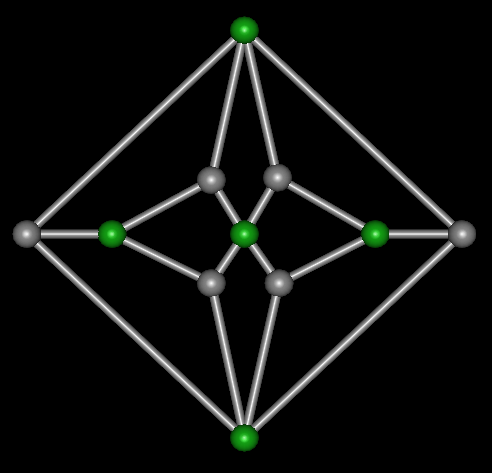
\includegraphics[width=0.4\textwidth]{img/herschel.png}
\caption{Grafo de Herschel, $n=11$, $k=5$, $k'=5$}
\label{fig:example-herschel}
\end{figure}


\subsection{O icosaedro}
Para o icosaedro~\cite{cite:example-plato},
apresentado na Figura~\ref{fig:example-icosaedro}.

\begin{figure}[htb]
\centering
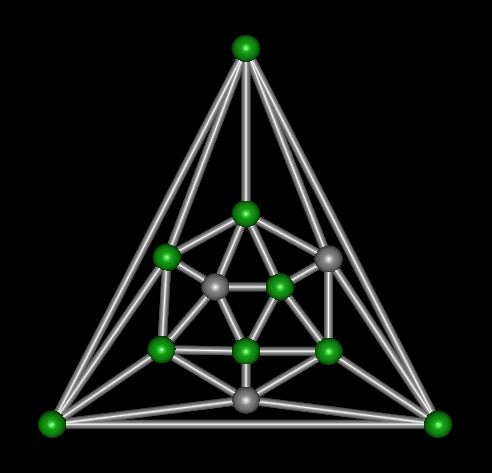
\includegraphics[width=0.4\textwidth]{img/icosaedro.png}
\caption{Icosaedro, $n=12$, $k=9$, $k'=9$}
\label{fig:example-icosaedro}
\end{figure}


\subsection{O grafo de Bondy-Murphy $G_3$}
Para o grafo de Bondy-Murphy $G_3$~\cite{cite:example-bondy},
apresentado na Figura~\ref{fig:example-bondymurphyg3}.

\begin{figure}[htb]
\centering
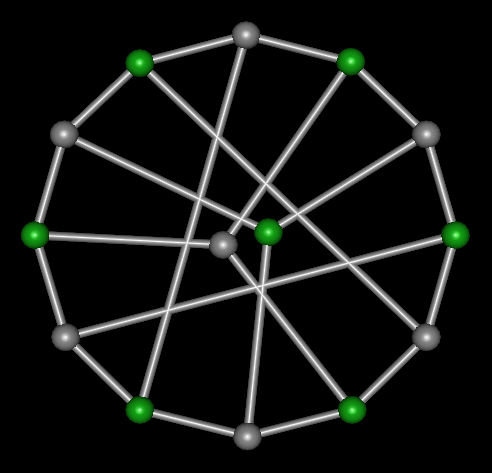
\includegraphics[width=0.4\textwidth]{img/bondymurphyg3.png}
\caption{Grafo de Bondy-Murphy $G_3$, $n=14$, $k=7$, $k'=8$}
\label{fig:example-bondymurphyg3}
\end{figure}


\subsection{O grafo de Bondy-Murphy $G_4$}
Para o grafo de Bondy-Murphy $G_4$~\cite{cite:example-bondy},
apresentado na Figura~\ref{fig:example-bondymurphyg4}.

\begin{figure}[htb]
\centering
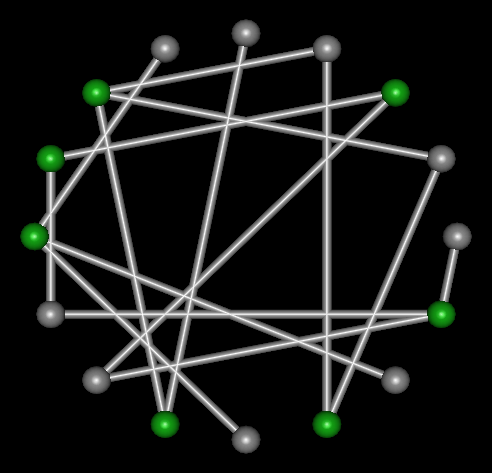
\includegraphics[width=0.4\textwidth]{img/bondymurphyg4.png}
\caption{Grafo de Bondy-Murphy $G_4$, $n=16$, $k=7$, $k'=7$}
\label{fig:example-bondymurphyg4}
\end{figure}


\subsection{O grafo de Ramsey $R(4,4)$}
Para o grafo de Ramsey $R(4,4)$~\cite{cite:example-ramsey},
apresentado na Figura~\ref{fig:example-ramsey}.

\begin{figure}[htb]
\centering
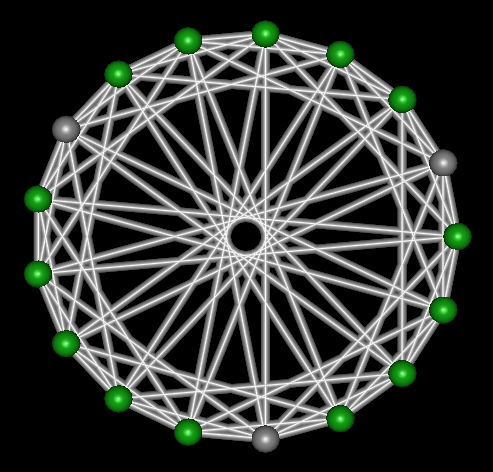
\includegraphics[width=0.4\textwidth]{img/ramsey.png}
\caption{Grafo de Ramsey $R(4,4)$, $n=17$, $k=14$, $k'=14$}
\label{fig:example-ramsey}
\end{figure}


\subsection{O grafo de Folkman}
Para o grafo de Folkman~\cite{cite:example-folkman},
apresentado na Figura~\ref{fig:example-folkman}.

\begin{figure}[htb]
\centering
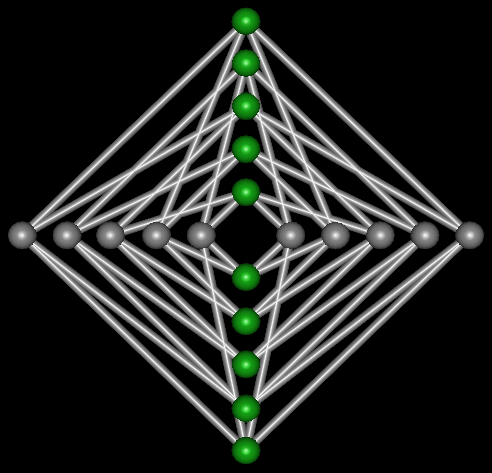
\includegraphics[width=0.4\textwidth]{img/folkman.png}
\caption{Grafo de Folkman, $n=20$, $k=10$, $k'=10$}
\label{fig:example-folkman}
\end{figure}


\subsection{O dodecaedro}
Para o dodecaedro~\cite{cite:example-plato},
apresentado na Figura~\ref{fig:example-dodecaedro}.

\begin{figure}[htb]
\centering
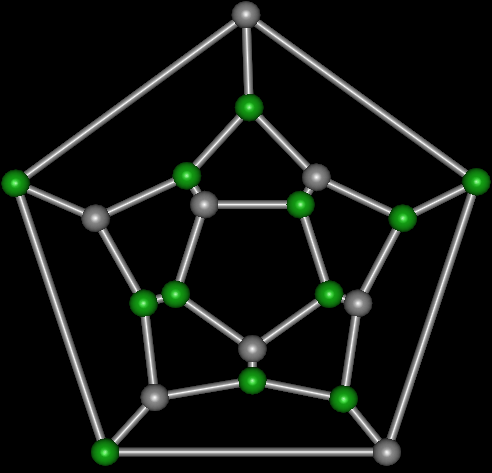
\includegraphics[width=0.4\textwidth]{img/dodecaedro.png}
\caption{Dodecaedro, $n=20$, $k=12$, $k'=12$}
\label{fig:example-dodecaedro}
\end{figure}

\subsection{O grafo de Tutte-Coxeter}
Para o grafo de Tutte-Coxeter~\cite{cite:example-tutte},
apresentado na Figura~\ref{fig:example-tutte}.

\begin{figure}[htb]
\centering
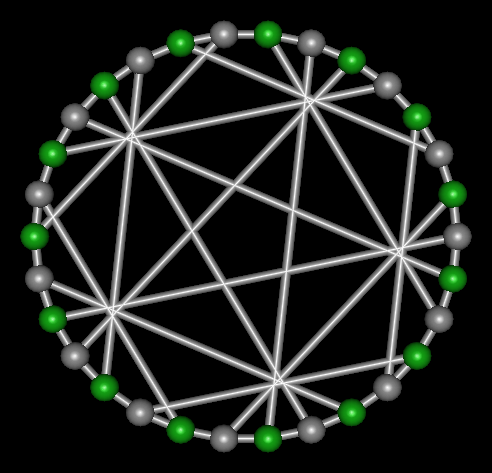
\includegraphics[width=0.4\textwidth]{img/tutte.png}
\caption{Grafo de Tutte-Coxeter, $n=30$, $k=15$, $k'=15$}
\label{fig:example-tutte}
\end{figure}


\subsection{O grafo de Thomassen}
Para o grafo de Thomassen~\cite{cite:example-thomassen},
apresentado na Figura~\ref{fig:example-thomassen}.

\begin{figure}[htb]
\centering
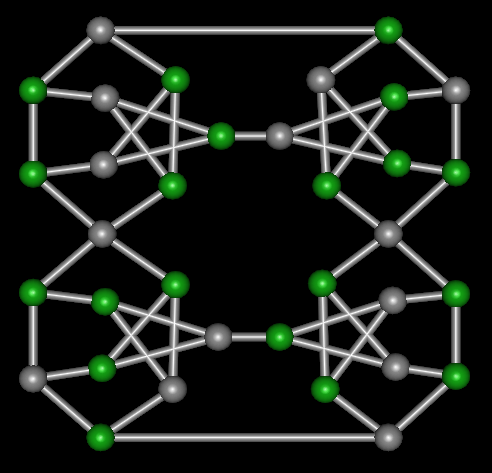
\includegraphics[width=0.4\textwidth]{img/thomassen.png}
\caption{Grafo de Thomassen, $n=34$, $k=20$, $k'=20$}
\label{fig:example-thomassen}
\end{figure}


\subsection{O grafo de Berge}
Para o grafo de Berge~\cite{cite:example-berge},
apresentado na Figura~\ref{fig:example-berge}.

\begin{figure}[htb]
\centering
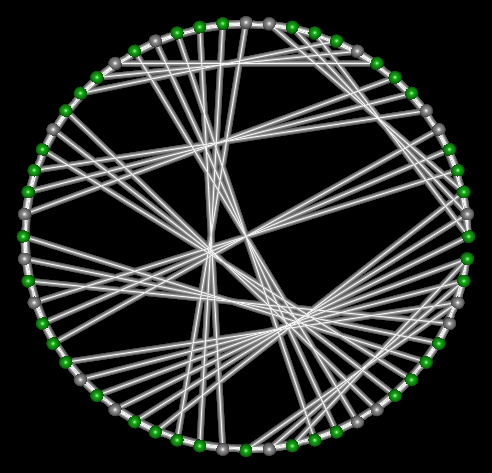
\includegraphics[width=0.4\textwidth]{img/berge.png}
\caption{Grafo de Berge, $n=60$, $k=40$, $k'=40$}
\label{fig:example-berge}
\end{figure}


\subsection{O grafo de Witzel}
Para o grafo de Witzel~\cite{cite:example-witzel},
apresentado na Figura~\ref{fig:example-witzel}.

\begin{figure}[htb]
\centering
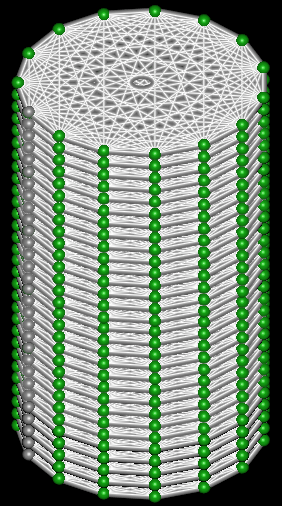
\includegraphics[width=0.4\textwidth]{img/witzel.png}
\caption{Grafo de Witzel, $n=450$, $k=420$, $k'=429$}
\label{fig:example-witzel}
\end{figure}

